
\documentclass[parskip]{cs4rep}
%\documentclass[bsc,frontabs,twoside,singlespacing,parskip]{infthesis}
\usepackage{graphicx}

\begin{document}

\title{Developing a Time Division Multiple Access Based Protocol for Efficient Data Recovery in Harsh Environments Through On Demand Dynamic Allocation of Bandwidth}

\author{William Pond}

% to choose your degree
% please un-comment just one of the following

\degree{Software Engineering}
%\course{Software Engineering}

% to choose your report type
% please un-comment just one of the following
%\project{Undergraduate Dissertation} % CS&E, E&SE, AI&L
%\project{Undergraduate Thesis} % AI%Psy
\project{4th Year Project Report}

\date{\today}

\abstract{
A novel solution to dynamic bandwidth allocation of static TDMA based networks at run time, specifically optimised for lossy channels with varying data rates, is investigated. The protocol is designed around unreserved bandwidth which is allocated on demand. As part of this protocol, an Automatic Request-Repeat (ARQ) sub-protocol and optimisations have been developed to maximise efficiency. The performance of the optimised ARQ and bandwidth allocation are presented in terms of throughput per node. It is found that dynamic bandwidth allocation in particularly lossy networks introduces large overheads which increase latency and decrease throughput. One conclusion is that it may be more appropriate to conduct profiling of harsh environments by building a series of static configurations.
}

%\section*{Acknowledgements}
%Acknowledgements go here. 
%This documentclass is a modification of the {\tt cs4rep} style that was formerly
%used in the Computer Science Department.

\maketitle

\tableofcontents

%\pagenumbering{arabic}

\chapter{Introduction}

This project has proposed and implemented a novel algorithm for the dynamic allocation of bandwidth at run time, on demand. Wireless sensor networks are becoming increasingly widespread and as the capabilities to develop and manufacture become more efficient, low power devices are realised. The project will focus on a specific part of this spectrum: motion capture. Motion capture is becoming increasingly popular with film and game studios; there is a high demand for ultra realistic computer generated imagery and models in games for which the data is generated from physical models. In addition to these motion capture also has uses in a wide range of other disciplines, such a medicine \cite{SPECK1} and sports analysis \cite{SPECK2}.

The project investigates a proposed protocol for motion capture in hostile environments, these vary wildly in their effects on the radio and abilities of the sensors to perform correctly. When operating in harsh environments there are a number of ways in which wireless sensors can be effected. For example moisture or small particles may come into contact with sensitive circuitry causing unexpected operation or breaking the devices. The project only focuses on a radio protocol, other protective measures are assumed to have been taken.

Attempting to perform motion capture on partially submerged bodies brings a unique set of challenges. As radio communications do not work under water unless using an extremely low frequency, most nodes will not be able to send data back until after the capture. At some points during the capture all nodes may be completly submerged and radio transmission stops entirely while at other points some nodes may leave the water for short periods. When nodes are very close to the surface of the water it is expected that there will be some successful data transfer over the radio, but this will be an especially lossy channel. 

Current methods for motion capture in industry can be broken down into optical and non-optical systems. Optical systems typically use a set of markers on the body and multiple cameras recording from different angles. The markers may be passive or active; passive markers (usually white spheres) reflect light in the room to the cameras whereas active markers may use LEDs or other technologies which the cameras can record. Once a sequence is recorded, post processing is required to map the location of each marker. Passive systems, such as inertial, take advantage of solid state accelerometers, gyroscopes and magnetometers and require less processing. As a result this processing can take place in real time. 

\section{Hardware}

The implementation developed in the project is for a specific hardware platform known as Orient 4, developed by the Centre for Speckled Computing at Edinburgh University \cite{W5}. This does not however limit the protocol to this hardware platform. The hardware assuptions are discussed later in the design chapter. The platform used includes an ARM Cortex-M3 processor manufactured by Energy Micro \cite{W1} along with a low power radio chip manufactured by Nordic Semiconductor \cite{W5}. The chip operates on the 2.4 GHz region of the spectrum, which is part of the range of frequencies freely licensed for WiFi networks. In addition to these the Orient 4 platforms contain a USB connector, which is controlled by the USB peripheral as part of the ARM CPU, thereby simplifying the development. These devices, known informally as specks, also comprise of multiple other sensors and modules to facilitate specific roles in research.

\section{Problem Specification}

Research has been performed into radio TDMA based networks but with dynamic slot assignment \cite{PR3} and although this does help to provide an understanding of methods for solving the problems faced, it does not directly access some particular issues encountered in this case. The sensor network consists of many mobile nodes and a single base station collecting the data and forwarding it on to a computer or other device where it will be stored for later processing and possibly real time processing. Communications are unidirectional for the most part, nodes transmitting sensor data to the base station. There is some scope for communication from the base station to nodes regarding assignment of extra transmit periods and calibration of on board sensors. It is therefore required that there are measures for the base station to communicate with nodes over a bidirectional link, although the bandwidth per node from the base station to the nodes is to be considerably less than that of the node to base station.

The configuration being proposed is in some ways similar to the cellular phone network, in which mobile phones communicate only with the base station and links are bidirectional. It does however differ with regards to roaming nodes. In the case of this project there will only be one base station and when nodes are not within radio range (due to distance from the base station or the medium preventing radio transmission, such as submersion in water), they are responsible for storing data until an appropriate time when transmission can resume. The major difference between this and the cellular network is that, unlike the cellular network in which nodes are often mobile and moving between base stations, there are a fixed number of active nodes which are all assigned to the same base station. This realisation does simplify the problem somewhat, the network topology used in this project is known and static.

The problem that this project attempts to solve is that of handling a fixed number of sensor nodes, or producers, running in real time and transmitting data back to the base station in lossy or unknown conditions. The base station, or consumer, must reliably receive as much data as efficiently as possible, while maintaining protocols for retrieving unreceived data. Additionally the project addresses issues such as time synchronisation for multiple clocks with unknown offsets and drift. As well as transmitting data, the protocol and implementation will also be required to reconstruct the data at the base station. This may be as part of the base station node or, more likely, the data should be sent straight to the computer attached to the base station where it will be reconstructed and processed. Additionally the base station computer should expose the reconstructed data through sockets to any other application wishing to process it in real time. The base station computer will be required to perform command and control of the network; for example its responsibilities will include starting a capture from the nodes, as well as issuing nodes with extra bandwidth in order to recover excess data as quickly and as efficiently as possible. This is in contrast to an ad hoc network in which there is no central authority controlling slot allocation.

\section{Implementation}

The protocol developed involves assigning each node a time slice for transmitting data back to the base station. During this time no other node may transmit, thereby eliminating the problem of packet collision. In addition to each node's time slice, or slot, a section of unreserved slots is created at the beginning of a capture. The base station acts as a central authority and is able to allocate these slots to nodes which require extra bandwidth. To provide delivery guarantees for data delivery an Automatic Repeat-Request (ARQ) protocol is incorporated into the network stack. The designed protocol was successfully implemented in full and validated as working. In addition to the dynamically allocated slots the ARQ protocol was optimised to provide a more efficient implementation in the protocol described.

\newpage
\section{Roadmap}

Related work and how it is integrated into this project is explained in chapter 2. Chapter 3 provides a full protocol description, defining what packets are sent and when; the chapter includes a full description of the network stack implementation. In chapter 4 the implementation is discussed, with an outline of the problems faced and their solutions. Experiments and their results are discussed in chapter 5. Finally conclusions and further work are examined in chapters 6 and 7.

\chapter{Related Work}

As mentioned previously there has been a wealth of research performed into networking, with specific reference to TDMA based networks and Automatic Repeat-Request (ARQ) protocols. These can provide some insight into building a system which makes use of many different protocols.  The following related work will be used to build up a set of protocols which complete the network stack required for this project.

\section{Time Synchronisation}

The most basic building block of a TDMA based algorithm is a solid time synchronisation protocol. Time synchronisation methods have been presented previously, including simple and low computation methods for calculating the clock offset and drift between two oscillators connected over a wireless connection. The methods presented by Sichitiu and Veerarittiphan \cite{PR1} propose a two way exchange of packets containing timestamps. When node 1 wishes to synchronise its timer to node 2, it sends a packet containing a timestamp according to the timer to be synchronised. When node 2 receives this packet it records the value of its timer in the packet. As soon as possible it returns the packet along with the value of its timer when sending. Node 1 now has 4 data points in order to evaluate its clock with relation to node 2.

Using these data points the paper presents two algorithms for calculating the clock offset and drift, by fitting the data points to two lines the relative offset and drift can be approximated by the offset and gradient of the line respectively. The paper presents a solution which discards data points which do not improve the accuracy of the estimations, known as Tiny-Sync. Finally the possibility of synchronising an entire network is discussed, which is the most applicable part to this project. It is also made clear that each node is able to calculate the time at the other node using these methods but does not necessarily modify its timer.

This method for time synchronisation may be more complex than required. Another method which uses reference broadcasts, known as reference broadcast synchronisation (RBS),  is most likely more suited to these requirements \cite{PR2}. The concept as stated is to broadcast a reference packet which can be received by all nodes. The time taken to queue, transmit and receive the packet is fairly consistent and can be corrected for. Elson and Estrin outline the method of performing this synchronisation and compare it to the Internet standard, Network Time Protocol (NTP). It is shown that RBS outperforms NTP by a considerable margin when implemented as a kernel module. In this project all modules have similar status to a kernel module as there is no operating system and all code is run in privileged mode. For this project a stripped down version of RBS can be used. The nodes clocks do not need to consider clock drift if the base station broadcasts at a short, regular interval. Additionally if the node has not received a reference broadcast in a set period of time it can be considered out of range of the base station and provided the clock drift upto this point is negligible the node can be considered always synchronised when in range of the base station.

\section{Bandwidth Allocation}

When using a TDMA protocol, bandwidth can be allocated in two ways: through changing the time slot length or number of allocated time slots to a single node. While both are suitable solutions to a network in which all participating nodes are always in range, increasing a time slot length is not viable in for this project. This is due to the fact that any change in a time slot length will impact all nodes. As such the only research of interest for this project is connected to the allocation of more time slots to single nodes.

Most research into dynamic slot allocation appears to include modifying the frame or slot lengths. For example the concept of multiple slot assignment is covered \cite{PR3} along with dynamic lengths. It is worth considering this paper as an example of slot allocation. The motivation for dynamic slot length in this paper is the nature of ad hoc networks and differing bandwidth requirements. When nodes enter the network they claim a slot. Nodes can also claim other slots if they require more bandwidth by announcing their intentions; the paper addresses procedures for allocating slots fairly if contention arises. The protocol for handling contentious slots is divided into three options, however all of the solutions include modifications to the timing lengths and such will not be considered for this project.

Obviously the biggest difference between this and the network to be implemented for this project is the nature of ad hoc networks. In the case of the paper, nodes must agree on all slot assignments as there is no central authority. The most important issue this paper raises is the concept of nodes being allocated multiple slots and releasing slots. Allocating multiple slots to a node is a common and straightforward task but allocating slots through a central authority has not been discussed. If each node is given one slot, and there are a fixed number of nodes which constitute the network then for this project, some slots can be kept aside and allocated to provide extra bandwidth on demand (as mentioned previously the frame length cannot be increased on demand).

If the idea of doubling frames is applied to doubling the slot length, it can be seen that rather than assigning a node many slots when more bandwidth is required the number of slots assigned to a node can be limited to a maximum of 2. Each node has its reserved slot and then can be assigned another slot from the unreserved pool. The leap in thinking is that rather than just assign one slot, the node can have multiple consecutive slots assigned or this could be considered as one slot with a length which is a multiple of the slot length, thus increasing the efficiency as intermediate guard periods need not be observed by the node.

\section{Aloha Protocol}

To complement the consideration of TDMA protocols, the Aloha protocol is considered as a solution to bootstrapping the network. It was developed to provide a solution to packet switched networks where TDMA and frequency division multiple access (FDMA) were unsuitable \cite{PR4}-\cite{PR5}. It does not require any bootstrapping to begin running and allows nodes to start up in any order, however traditionally it does require full duplex radios. It may also be suitable as it would allow the network to start up with many nodes, and then only nodes to be used as sensors can be sent the TDMA information, thus allowing some control in the setup of the network, without concerns of nodes not participating in the capture of data taking up valuable TDMA slots.

The basic principle of the Aloha protocol is that when a node has data, it should attempt to send it. If there is a collision the node should wait a random amount of time before retrying. This concept is simple enough to implement but in the case of this project will require some modifications. For instance, the sending node is not aware of any collisions, therefore acknowledgements in some form must be included. Additionally generating random numbers on embedded devices is another problem which can be avoided by using the unique serial of each processor.

\section{Go-Back-N ARQ}

The Go-Back-N (GBN) ARQ is a sliding window based protocol which provides a packet delivery guarantee, as required for receiving data from the nodes. The basic principles are outlined by Figure~\ref{fig:GBN}. A frame, or window, size is agreed before transfer begins. The sender transmits the the window size number of packets and then waits for acknowledgements from the receiver. The receiver receives these packets, sending an acknowledgement for each packet received. As the sender receives these acknowledgements the window of outstanding packets is incremented. If the sender does not receive an acknowledgement after some timeout period, the window is reset to this packet and transmission reoccurs. Yao \cite{PR6} presents a method for achieving higher throughput on connections in which there is a high error rate; the solution presented suggests that there are two modes of operation, low and high error rate. In the high error rate, packets are transmitted n times to ensure delivery. The concept is that the GBN implementation regresses to a Stop-And-Wait (SW) ARQ if there is poor throughput \cite{PR7}.

It certainly appears as though the GBN implementation may be a suitable candidate ARQ scheme. With some modifications this scheme may be optimised for the project, for instance if the window size is defined by the maximum number of packets which can be sent during one frame (the total number of packets which can be transmitted during all of the nodes transmit time as defined by the TDMA schedule) a single acknowledgement could be provided by the base station, thus reducing the overall network load. Additionally it may be more efficient to group acknowledgement packets from the base station.

\begin{figure}
	\centering
	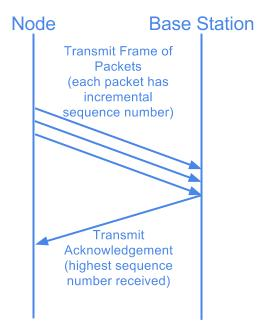
\includegraphics[width=60mm]{gbn.jpg}
	\caption{Proposed Go-Back-N ARQ Process.}
	\label{fig:GBN}
\end{figure}

Additionally the proposed acknowledgement scheme may be required to send multiple copies of the acknowledgement packet to ensure delivery, similarly to the data packets sent with the SW ARQ. If the packet loss on the network is high, a single acknowledgement packet may be lost resulting in a high latency for packet transmission (and possibly large queues on the sender) due to the slotted nature of TDMA.

\chapter{Protocol Design}

The protocol must handle high rates of packet drop and changes in network topology. The network is split into nodes and a base station. Nodes may leave and enter the network at any time but there is always a fixed number of nodes taking part. As a result the protocol must provide an efficient use of the time in which nodes are within range of the base station. The protocol described is split into two sub-protocols for transmitting packets (Aloha and TDMA) and then into a network stack for handling control and data messages.

Nodes are given an ID when programmed. Each node taking part in any network created must have a unique ID as this is used to address packets to the node. This is suitable for the project as when performing motion capture the position of each node on the body must be known in order to interpret the data correctly.

\section{Hardware Assumptions}

The protocol makes some assumptions related to the hardware available; the physical layer is implemented in a form which handles error checking (in this case CRC), transmission and receiving of single, fixed length packets. It is assumed that the radio implementations perform broadcast based communication and therefore addressing is managed by the network stack. Additionally it is assumed the radios used are half-duplex and can only transmit or receive at any one time.

The described protocol attempts to take into consideration the nature of the other hardware available. As these nodes are often small in size and restricted in available hardware (if only to maximise battery life), the protocol must take into account measures for time synchronisation as well as clocks with a limited number of hardware interrupts. It is assumed that the hardware available is, however, capable of performing accurate hardware interrupts based upon time (interrupts to the processor and from the radio chip).

\section{Aloha}

Based on the AlohaNet \cite{PR4}, \cite{PR5} protocol built in the 1970s, the network is bootstrapped using this protocol. The implementation used is adapted to the available hardware. Every time a node receives a packet the local time is recorded. If a node wishes to transmit a packet the last receive time is inspected, should there have been sufficient time between the last receive time and the current time, the node changes to transmit mode and sends the packet. If the last receive time was within a predetermined time period, the node must wait until the timeout before transmitting. If another packet is received during this time, the node must reset it’s timeout. The timeout value is pseudo-random for each node, it is a function of the time at which the on-board CPU was programmed. This time stamp of manufacture is stored on the CPU as part of the unique processor identifier. As the hardware is assumed to be half duplex the node is unable to tell whether a collision occurred during transmission and it is therefore the responsibility of the higher levels of the network stack to implement retransmissions if and when required.

Nodes in Aloha mode remain in a receiving and ready state for instructions from the base station. Generally radios see significant increase in power consumption when receiving as opposed to transmitting or in standby. The network must be conscious of power consumption and as such it is not intended for nodes to remain in Aloha mode for extended periods to preserve the battery life of each node.

\section{Time Division Multiple Access (TDMA)}

TDMA has been used for sensor networks to transmit data in previous research \cite{PR3}, \cite{RFC1}, \cite{RFC2}. This is the mode used during the main operation of network. It provides a Medium Access Layer (MAC) layer guarantee that radio transmissions will not collide. As a result of TDMA each node has a synchronised clock which is available to applications for time information. The TDMA protocol outlined in this sections is adapted from a static network to provide additional bandwidth to nodes when requested in order to fulfill changes in requirements. As there is a fixed number of nodes in the network, but these nodes are expected to leave the range for unknown durations a static solution may not be able to meet later bandwidth requirements as nodes rejoin. Additionally when nodes rejoin the network there may be a large amount of data produced which must be transmitted as efficiently as possible.

Each node must be given the following to initiate their TDMA mode:
\begin{itemize}
\item
Radio channel - the radio frequency to use for TDMA mode.
\item
Slot - the slot to use for transmission (from the reserved section).
\item
Slot count - the total number of slots available (from which the TDMA frame period can be calculated).
\item
Guard period - the time between consecutive transmit periods.
\item
Transmit period - the time in which a node may transmit.
\item
Protection period - the time a node must allow before the end of the transmit period for it’s hardware buffers to empty. During this period the node must not send any more packets to the radio hardware but is still considered to be in the transmit period.
\end{itemize}

\subsection{Outline}

\begin{figure}
	\centering
	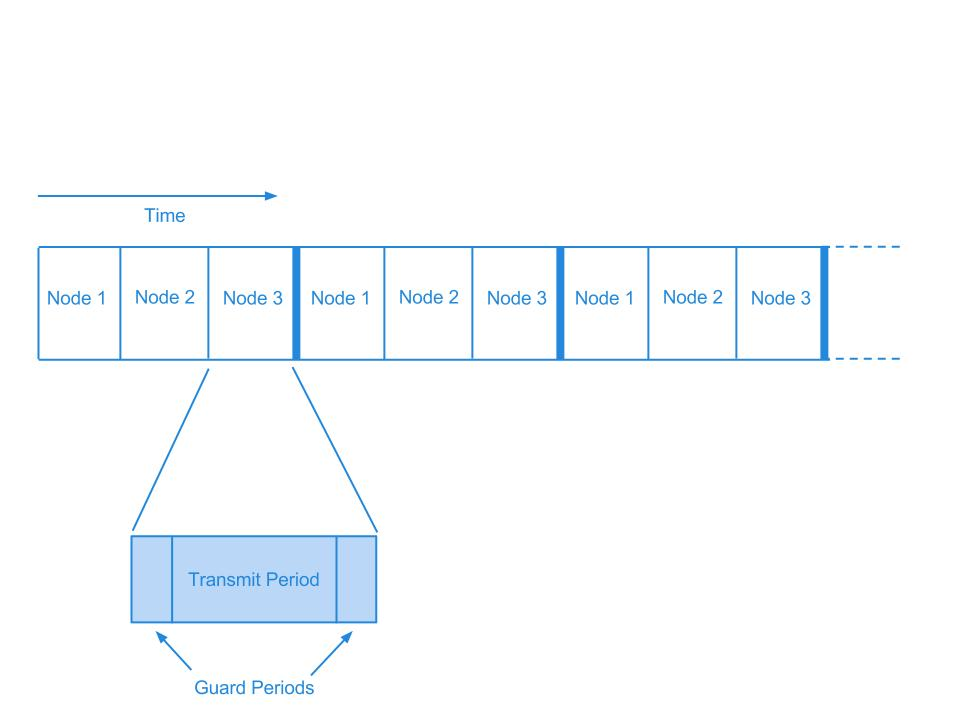
\includegraphics[width=120mm]{tdma.jpg}
	\caption{Basic TDMA.}
\end{figure}

The network is started in Aloha mode; when each node starts it is in a receiving mode, waiting for packets from the base station. The base station may send several combinations of packets (described later) to inform the node of it’s TDMA configuration and instructing it to change to TDMA mode. Once in TDMA mode, each node owns one slot in the reserved section. TDMA requires a method for synchronising the clocks of all participant nodes, described in this section is the method of Reference Packet Synchronisation for distribution of timing information from the base station to nodes.

When data packets are transferred by the higher levels of the network stack, a request for more bandwidth may be included. If this request occurs the base station allocates one or more consecutive slots from the unreserved section. These slots are leased to the node and may be renewed after a set number of TDMA frames. A TDMA frame is defined as the time between adjacent broadcasts of the timing packet.

\begin{figure}
	\centering
	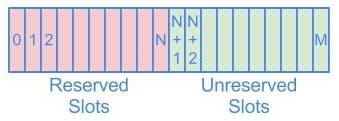
\includegraphics[width=80mm]{slots.jpg}
	\caption{Slot Reservations.}
\end{figure}

The reserved section is comprised of the slots from zero to N, the node count (the base station must always use slot zero, and each participating node is allocated one slot). The slots from N+1 to M comprise of the unreserved section. Slots from this section may be leased to nodes when required as described in the dynamic slot allocation section.

\subsection{Reference Packet Synchronisation}

It is assumed that the base stations clock is absolute; the drift and offset of the base station are zero. In actual fact this is not true as the clock on the base station suffers the same drift as the clocks on the nodes.

The base station transmits a reference packet \cite{PR1},\cite{PR2} at the beginning of each TDMA frame. The reference packet does not contain any timing information, the time of receipt and the known time of transmission is the only information required for synchronisation. By reducing the timing information in the packet, less input is required from the CPU and therefore there is less chance of inaccurate timing information. Each TDMA frame, the base station queues a single timing packet and activates the radio through a hardware interrupt at the beginning of its transmit period. When a node receives this packet, an accurate time of receipt is recorded using another hardware interrupt (when the radio triggers an interrupt, the timer records the local time this happened). Through this the node can synchronise its clock to match the base stations.

If a node does not receive a timing packet, it is assumed that the clock drift is within tolerances and the node continues to transmit during its perceived transmit period. If a node misses a series of timing packets (in this case 3) it must cease transmission until a time at which it begins receiving packets again. If a node is not currently receiving timing packets it is considered out of sync. During this time the node remains in receive mode until a timing packet is received. When a timing packet is received the node returns to TDMA mode, utilising only it’s reserved slot (any slots dynamically allocated are discarded as the lease for this slot may have expired).

\subsection{Dynamic Slot Allocation}

As nodes will vary in their demand for bandwidth, the base station must be able to dynamically allocate radio time to nodes as required. It is intended that the slot allocation from the reserved section will be suitable for normal operation (the node remains within radio reception of the base station and there is little or no interference which could cause excess packet loss) such that the node does not produce more data than can be transmitted. If this is not the case, the slot period must be extended to allow this.

During TDMA operation each node is expected to report the state of its buffers through the transport layer. Flags are used in the transport data packets to signal buffer fill and if the base station receives packets from a node indicating its buffers are either almost full (in this case over 75 per cent full) or overflowing (the node is using external storage for new data) extra slots may be leased to the node.

In order to simplify the implementation on embedded hardware (and to make the most efficient use of hardware timers available) the dynamic slot allocation is restricted to one slot from the unreserved section. However, the length of this slot may be a multiple of the slot period and as such nodes may be allocated any number of consecutive slots. When a slot is allocated, it is leased to the node for a preconfigured number of TDMA frames, the motivation for this is that if the node leaves radio range, the slot can be reassigned after this time without further contact.

A series of slots has a lease length equal to the shortest lease of one of the component slots.  When a lease is generated, the information is sent to the node and an acknowledgement must be sent by the node when it receives this. During the time between lease creation and acknowledgement the protocol it is assumed that the node is using the slot. In this description of the protocol it is assumed that once a node has been allocated it will be leased for the duration regardless of acknowledgement. Acknowledgements are especially important for configurations in which nodes are given long leases to ensure slots are utilised properly. It is recommended that lease times are kept short as slots can always be reallocated if required and this is better for slot contention.

\subsection{Limitations}

The main limitation with the TDMA protocol described is the top values for the hardware timers. The protocol does not provide measures for dealing with timers which have an overflow period less than the desired period for the TDMA period (the reserved and unreserved periods). It is assumed that suitable hardware scaling of the clocks can be used in order to overcome this issue or that TDMA period will be restricted.

Nodes use their ID as their address, there is therefore a limitation of 253 nodes on any subnet as in packets addresses are limited to one byte. Additionally the base station must be allocated address 0 and broadcast packets are given address 255.

\section{Network Stack}

The implementation of the algorithm is split into a 3 layer network stack consisting of the physical layer, network layer and transport layer. The network layer provides a service for sending packets with no delivery guarantees. It also provides the means to send and receive control and event packets. These packets will be described in full in the Packets section. The network layer also contains an event system. Events consist of one byte identifiers and can be sent to any node. Above the network layer is the transport layer; the transport layer is responsible for providing delivery guarantee for data. It does not however provide any timeliness guarantees.

\subsection{Physical Layer}

The physical layer in this case comprises of the radio hardware and hardware protocols for accessing it by the CPU. It is expected that the hardware buffer available on the radio module will be not be suitably large to contain an entire slot worth of data. The physical layer will not be expected to implement the extension to the physical buffer but will write directly to it. It is expected that the network layer will implement a queue of packets.

\subsection{Network Layer}

The network layer consists of a packet queue which is written to by the physical layer, when a packet is received by the radio it is written directly into this queue. This however may be different between implementations. When the transport layer wishes to receive a packet, the queue is inspected. The next packet in the queue is considered, if it is a control or event packet it is consumed by the network layer (and any resulting action is taken). When a transport layer packet is found, the contents are copied into a supplied buffer, freeing this space in the queue.

\subsubsection{Event System}

It is intended that the event system is used for simple communication between base station and application. For instance the event system may be used to trigger the start/end of data capture or calibration modes. Event packets are not acknowledged and any required acknowledgement of an event must be handled by the application. When events are received they are queued, in order, before being passed to the application for processing. Up to 30 events may be transmitted in a single packet as a null terminated list (if all 30 bytes are used the list will not be null terminating). The application is expected to poll the events queue periodically and handle any events which have been received in a timely manor. There are two reserved events for communication of state information between the base station and computer.

\subsection{Transport Layer}

The transport layer uses an Automatic Repeat-Request (ARQ) protocol based upon Go-Back N \cite{PR6}, \cite{PR7}. The size of the window is intended to be the number of packets which can be transmitted in one TDMA frame. As such the window size is actually dynamically varied based upon slot and therefore bandwidth allocations. When an application sends a block of data, this is considered a transport frame. A frame is broken down into segments of 25 bytes, with a maximum of 256 segments (as the segment ID is one unsigned byte) and therefore a maximum of 6.25 KB per frame. The transport layer queues these segments in its internal buffer. In this implementation, the transport layer must consist of a separate internal buffer to the network layer as after transmission the network layer is expected to remove the packet from the queue. As such each TDMA frame the transport layer must refill the network layer queue with the current packets to be sent. On receipt of a transport acknowledgment packet, the transport layer steps through the packets in its buffer, removing packets which have been successfully sent.

\section{Packets}

The following is a description of the packets used by the protocol. The packets have a common packet header compromising of two unsigned bytes, address and type. Additionally packets are of fixed length and are described for a length of 32 bytes. However this could be extended to include larger packets if hardware allows, with the minimum packet size being 20 bytes. Any decrease in packet size a direct relationship with decrease in maximum frame size. Each packet listed below has a unique packet type identifier.

\subsection{Timing}

The timing packet is reserved for the reference packet time synchronisation protocol described earlier. This packet is only broadcast during TDMA mode and does not require any kind of acknowledgement from nodes. A packet with the timing ID may only be broadcast by the base station and must use the broadcast address.

\subsection{Hello}

The hello packet is similar to a ping. Any node may send an hello packet addressed to any node or the broadcast address. When a node receives a hello packet, it broadcasts a reply containing its ID. The hello packet is intended to be used by the base station to discover the presence of nodes during the bootstrapping phase of the network. The hello packet contains a unsigned one byte field known as the ChallengeResponse field. This field must have a value of 255 when an hello packet is sent. When a response is received this field will contain the ID of the sending node.

\subsection{TDMA Configuration}

The TDMA configuration packet must only be sent by the base station (which is the TDMA authority) and must contain the following information:

\begin{itemize}
\item
Sequence number (1 byte unsigned) - this number is used by the node to acknowledge receipt of the packet.
\item
TDMA master flag (1 byte boolean) - if a node is set to the TDMA master it sends the reference packet for timing. This is only set to true when configuring the base station.
\item
Channel (1 byte unsigned)  - the radio channel to be used for TDMA. It is intended that the TDMA mode use a different channel to the aloha mode in order to minimise collisions and interference from nodes not participating.
\item
Slot (1 byte unsigned) - the slot index to use for transmission.
\item
Slot count  (1 byte unsigned) - the total number of slots available. This is used to compute the total period of one TDMA frame.
\item
Guard Period (4 byte unsigned integer) - the time between adjacent transmit periods.
\item
Transmit Period (4 byte unsigned integer) - the time allocated for the transmission of packets.
\item
Protection period (4 byte unsigned integer) - the time allocated at the end of transmission for the hardware buffers to empty.
\item
Enable flag (1 byte boolean) - whether to enable the TDMA configuration. It is expected that this will normally be true but there may be cases in which the configuration will be distributed and then an enable signal sent at a later time.
\end{itemize}

When a node receives a TDMA configuration packet, the node must reply with an acknowledgement (TDMA ACK) containing the packets sequence number. This acknowledgement may be used by the base station to confirm the receipt or that the actions as a result of this packet are being performed (i.e. the node is moving to TDMA mode).

\subsection{TDMA Enable}

The enable packet is similar to the configuration packet but does not contain configuration data. This packet is intended to be used once nodes have been configured. For instance if the base station wishes to move all nodes from TDMA mode back to Aloha mode this packet may be broadcast. Similarly to the TDMA configuration packet, a node must return an acknowledgement packet (TDMA ACK) on receiving this packet. The packet consists of a 1 byte boolean instructing whether the TDMA mode should be active or not and a 1 byte unsigned sequence number which must be returned in a TDMA ACK.

\subsection{TDMA ACK}

The acknowledgment packet comprises of a single one byte unsigned sequence number. When a TDMA packet is received by a node, this packet will be returned to the base station. This packet is not acknowledged.

\subsection{Transport Data}

The transport data packet contains headers detailing the contents of the packet. The packet also contains flags which communicate the state of the buffers, explicit requests for slots and the end of frame flag. It is intended that transport data packets are sent by nodes and received by the base station. The packet contains the following fields:

\begin{itemize}
\item
Sender ID (1 byte unsigned) - the ID of the node from which this packet originated.
\item
Frame ID (1 byte unsigned) - the ID of the frame this packet belongs to. A current frame can be uniquely identified by the sender ID and frame ID. The frame numbers must start at 0 and be incremented by one each time a frame is created.
\item
Segment ID (1 byte unsigned) - the ID of the segment. The segment ID must start at 0 and be incremented by each segment queued.
\item
Segment fill (1 byte unsigned) - the number of bytes in this packet. If this is the final packet this may be less than the number of bytes available for the payload.
\item
Flags (1 byte unsigned) - any combination of the following flags
\begin{itemize}
\item
0x01 - final segment
\item
0x02 - buffer level high (> 75 per cent)
\item
0x04 - buffer full
\item
0x08 - external storage full
\item
0x10 - unused
\item
0x20 - unused
\item
0x40 - unused
\item
0x80 - explicit request for slot (this may be honoured by base station)
\end{itemize}
\item
Segment payload (25 bytes)
\end{itemize}

The base station must not acknowledge each transport data packet but must transmit one acknowledgement each TDMA frame to each node from which it has received data from in the previous tick.

\subsection{Transport ACK}

The transport ACK packet contains the acknowledgements from the previous TDMA frame. As the base station is always ID 0, each node will receive any acknowledgments before their slot and therefore have time to remove any successful packets and only send new data. The transport ACK packet also contains details of a second slot for the node, as extra bandwidth is only required when nodes are sending data it is logical that extra bandwidth assignments should be bundled with the transport acknowledgment. The following fields are available in this packet:

\begin{itemize}
\item
Last frame ID (1 byte unsigned) - frame ID from the last packet accepted by the base station.
\item
Last segment ID (1 byte unsigned) - segment ID from the last packet accepted by the base station.
\item
Second slot flag (1 byte boolean) - whether the following information contains details of a second slot.
\item
Sequence number (1 byte unsigned) - the sequence number relating to the slot allocation.
\item
Slot ID (1 byte unsigned) - the second slot index the node has been allocated.
\item
Length (1 byte unsigned) - the multiple of slots for which the node can transmit.
\item
Lease (1 byte unsigned) - the number of TDMA frames for which this slot allocation is valid.
\end{itemize}

When a node receives a transport acknowledgement containing details of a second slot, the node must return a TDMA ACK containing the same sequence number.

\subsection{Event}

The event packet contains a null terminated series of 1 byte event identifiers. The event packet is consumed by the network layer. When events are received the node queues these in order and supplies them to the application.

\section{Base Station}

The base station is connected to a computer via USB configured to appear as a serial connection. A packet switched layer is built upon this to allow efficient communication. Normally the base station is intended to be a dumb relay for packets to and from the nodes, with the computer creating and sending most packets. It is therefore logical that packets of 32 bytes are used between the computer and base station (or the same length as used in the radio implementation). It is also required that the computer can send instructions directly to the base station, therefore the base station will consume all packets which are explicitly transferred with address zero. As a result the base station will send all packets over the radio which are not addressed to it and send all packets received from the radio to the computer.

It is also expected that the computer will know the state of the base station and as such there are two reserved events which the base station must send to the computer. The first is a TDMA frame event, which is dispatched each time the main clock overflows. The second is a packet sent event which is dispatched as a packet is transferred to the radio module. As the speed of the connection to the computer is expected to be much greater than the radio connection and the base station is expected to be externally powered, the bandwidth concerns of nodes are not present for the base station.

\chapter{Implementation}

The Orients feature the standard speck modules in addition to a micro USB connector, SD card reader, magnetometers, gyroscopes and accelerometers. These sensors are used along with an adaptive quadrature algorithm to determine the Orient's rotation in 3D space. For this project only the USB connection, radio and processor will for development and testing. 

\section{Structure}

\subsection{Timers}

The timers, of which there are 4 on the chip, are a part of the peripherals packaged by Energy Micro which are on the chip die but not part of the ARM processor core itself. Throughout the implementation of the project the timers on the processor have taken a key role in achieving a working implementation. Obviously for a TDMA protocol all nodes must have synchronised timers and as such these were the first cause of problems during the project. The timers can be configured to interrupt the processor at a specific time or record the time an event took place (the polarity of an input pin changes) and interrupt the processor. There two configuration form the basis for the TDMA protocol. The timers must be configured to enable the radio at specific times and record the time of receipt of specific packets. While these may seem like a standard and fairly simple use of the timers, they do introduce their own problems. The processor must be able to control the radio chip to configure, enable, disable it etc. however the timers also need to be able to interface with it. As such race conditions exist which have caused numerous minor problems. This was overcome by carefully distinguishing the roles of the timers and processor in interacting with the radio; some of the control is now routed through the timers which alert the processor to what has happened rather than the processor attempting to control the interface directly. 

\subsection{Radio}

The processor communicates with the radio through a USART serial interface which provides synchronous serial communication at a maximum data rate of 8 mbps. The USART is a peripheral of the processor, while not in the ARM processor core it is part of the processor package. There are three techniques for interfacing with the USART peripheral and the radio chip, implementations using all three were attempted during the course of the project and their methods and reasoning will be explained further. The USART peripheral has a two one byte buffers, in the case of transmission one is written to by the processor while the other is read over the serial connection. The aim of this is to minimise time between sequential bytes being sent and therefore maximise the data rate. 

\subsubsection{Direct Control}

The processor takes full control of the USART peripheral and writes each byte to the next buffer as it becomes available. While waiting for the buffer to free up the processor enters a waiting state for the current byte to complete transmission. This is obviously a waste of processor time and power however it is useful in some situations, for instance throughout the project this technique has been used during the startup of the system, to set the configuration registers of the radio. The first implementation of packet transfer over the radio used this technique. 

\subsubsection{Interrupt}

Each time the USART peripheral has written a byte an interrupt is raised with the processor, which can then write the next byte to the buffer. This has obvious improvements over direct control from the processor as it introduces a form of parallelisation to sending data. This technique was used when looking for faster alternatives to direct control by the processor. 

\subsubsection{Direct Memory Access Peripheral (DMA)}

The final method for communications is to use the DMA, another peripheral of the processor. The DMA has access to the processor's memory and as the USART peripheral is also mapped to the processor's memory, it can be used to perform transfers with no interaction from the processor. This is especially important if speed is a priority and as such an implementation using this peripheral was attempted. By including this peripheral in the project many problems, specifically in debugging, are introduced. As it is not part of the core execution of the processor any tasks which are given to it for it to perform happen completely in parallel; one could consider the DMA as a black one - memory addresses are put in and an interrupt is raised when the operation is complete. Regardless of these obstacles an implementation was completed using the DMA which will be discussed shortly. 

\subsection{Radio Implementation}

The project went through several key iterations of development mainly due to lack of understanding of some of the hardware causing unknown or inexplicable bugs. Development of the project was performed in an iterative basis; first sending and receiving packets correctly over the radio was implemented, then the basic TDMA, followed by the ARQ and finally the functionality for nodes to realise and use unreserved slots. During the first few iterations using direct control and interrupt based control it was found that the processor actually gave fairly poor performance of throughput. A solution involving the DMA was used which provided much faster throughput but introduced a large amount of unexplained packet loss. Eventually it appeared that this packet loss was caused by interacting with the radio chip too quickly - the processor would queue the next DMA transfer so quickly that the radio chip was unable to process the current packet. Once this issue was isolated and delays added the TDMA functionality was added. This involved building a separate module which controlled the timers and could interact with the radio where required. 

The development of the TDMA functionality incurred more problems, as outlined in the timers section. Initially the system for this involved registering functions to be called with their related times. The next solution involved performing the operations in the timer interrupts, while this ensured little latency between time of interrupt and code execution it can have detrimental effects on other time sensitive interrupts. The system worked during normal operation but introduced many more bugs related to race conditions especially when combined with the DMA and radio interrupts. A less elegant but simpler solution was found by setting a state flag and handling these on state change in the main function. By using this method with sequentially numbered flags and a switch/case the compiler generates a lookup table which gives good execution time. 

As a result the final version included a simplified version of the radio driver too, a version using only direct control by the processor was chosen. This minimised the number of problems relating to the complicated ARM interrupt system (known as the Nested Vectored Interrupt Controller or NVIC) and issues relating to the speed associated with the DMA. By rolling back to the more simple setup the protocol can be tested with confidence that no unknown race conditions will manifest as dropped packets or loss of synchronisation.

\subsection{Reference Packet Synchronisation}

Synchronised clocks are a requirement of any TDMA algorithm and this is achieved through the  reference packet method described in the related work section. The actual implementation of this however is slightly more complex as the nodes cannot be sure which packet received will be the reference packet. When a node requires synchronisation, it changes to receive mode, checking every packet received for the reference packet. When this packet is found, the node goes into a partial TDMA mode. As the node knows the time interval between two reference packets and the reference packet is sent at the beginning of the base station's transmit period, the node can wait to record an accurate time for the next reference packet. This is done by loosely synchronising the clock; the synchronisation is only accurate enough to ensure it starts receiving a short time before the next reference packet. Once the node has received that reference packet and synchronised its clocks the full TDMA mode can start; the difference between the full and partial TDMA mode is that the node does not recognise its reserved slot, and thereby transmitting no packets, to ensure there are no collisions from the loosely synchronised clock.

\subsection{ARQ}

As discussed earlier, when data is ready to be sent by the node, it is considered a frame. Each frame is broken down into fixed size segments, ready for transmission. When the node splits a data frame into segments, each one is queued in order. When the base station receives a data packet, it checks if it is the next packet received, if not then it is discarded. At the start of each frame the base station sends an acknowledgement to each node with the last successful frame ID and sequence number. When a node receives this acknowledgement it removes all packets in the queue which have been successfully sent. 

When a packet is received and accepted as the next expected packet it must then be put together with the other data which makes up that frame. If a segment has the end of frame flag set, it indicates that the next packet to be received will be the next sequential frame. Each packet also contains a count of the bytes it contains, the main motivation for this is to instruct the base station how many bytes are in the final packet of a frame. While intermediate packets could contain less than 25 bytes, there is little point and as such it is not supported in the implementation. When a packet is successfully accepted by the base station its frame and sequence numbers are stored in a lookup table which is used when generating the acknowledgements.

Acknowledgements are generated by the base station, on demand. When the base station is in transmit mode and ready to transmit the next packet, it traverses the lookup table for the next node to send an acknowledgement to. If it finds a node it generates and sends the packet. In addition to the acknowledgement a slot allocation may piggyback on the packet, these are generated at the same time. If a node has an outstanding allocation, one which has not been acknowledged, the details are resent. 

\subsection{Slot Allocation}

If a node either has high buffer levels or requests extra transmit time, a slot may be allocated when generating an acknowledgement. Slot allocation is performed by a separate module (as it has no hardware dependencies, only request and get methods, allowing separate unit testing to be performed) which stores a lookup table of slots, the node they are allocated to and the remaining lease. As nodes may only occupy one slot with a length which is a multiple of the slot length, the system should avoid allocating adjacent slots where possible. When a node requests a slot, the first action to perform is to check that whether the node has an existing slot. If it does then the algorithm attempts to allocate an adjacent slot. If the node does not have a slot the next free slots is shown by stepping through the slots leaving a predetermined gap between each slot to allow for adjacent allocations. 

\subsection{USB}

The USB driver is one of the most important parts of the project, it is responsible for sending data from the base station and debug messages from the nodes to the PC. The USB driver was supplied as part of the Energy Micro USB stack \cite{W1}, some changes were made to make it more efficient. The driver provided a CDC interface which means it presents as a serial interface to the operating system on the PC. Initially a circular buffer was implemented, when data was ready to be sent it was copied into the buffer and sent either straight away or after the current operation has completed. The USB peripheral requires buffers with a 4 byte alignment, which cause some problems with sending data part way through the circular buffer. As a result a second, transmit buffer, was used; data was copied out of the circular buffer and into the transmit buffer before sending. Obviously this comprises of two copies of the data before sending and is not efficient. There were many problems with USB efficiency throughout the project which will be discussed further in the base station section. The final iteration of the USB module used two large buffers, both correctly aligned for the USB peripheral. One buffer is used for writing and the other is read by the peripheral, through this method data is only copied once to a buffer then sent. 

\subsection{Base station}

The base station also took several forms through the course of the project. For the most part the base station was a Python implementation using the pySerial library to provide the serial connection \cite{W2}. The core Python base station included a command line style control of the network, nodes could be moved between Aloha and TDMA mode as well as send events and displayed data rates for received data packets. Originally the Python base station was also responsible for generating the ARQ acknowledgements, however it was discovered that due to the Python Global Interpreter Lock (GIL) \cite{W3} combined with the operating system's scheduling of threads, some acknowledgements were not passed to the base station in a reasonable amount of time. This is also consistent with the fact that the USB transmissions are handled by the operating system and may not happen straight away. A solution was developed using a C based serial library \cite{W4} which provides cross platform functionality. Unfortunately, unlike the Python solution, the implementation of this is not cross platform and therefore currently is only available on Microsoft Windows.

\section{Testing}

During development of the firmware, a combination of the following 3 techniques were used to test the execution of the firmware. The first and most simple method was using the LEDs. This was mainly used before the USB was working correctly and as there were 3 available LEDs there exists 8 combinations available to display. LEDs are still used during execution for warnings; for example the red LED is illuminated if the USB buffer overflows, as buffer overflows are not always obvious from the logs. The next form of debugging available is using the USB and an ASCII serial connection viewer to send text based messages back to the computer. Finally step by step and hardware breakpoints were used via GDB and J-Link. As the implementation relies on the hardware and its peripherals the code cannot be executed or simulated on a computer, but a combination of text output and step by step execution provides a high level of confidence that the system is working. As the system is highly time sensitive text based output is preferred and wrapper functions were written to include the value of the timer with the message. 

\section{Validation}

It is important that the protocol is shown to be operating correctly, as such the procedures used to ensure it is working correctly are outlined below. The main procedure was to generate logs, each line includes a timestamp and message\footnote{Sample node logs are available in appendices A-C. The full versions of these node logs were submitted with the code.}. In addition to the timestamp in the debug messages, the number of times the timer had overflowed was also recorded. Some bugs were discovered with the USB driver which caused processor stalls for whole cycles of the timer. Bugs such as these motivated the move from Python to C as it was discovered Python was not polling the base station USB connection with a high enough frequency to prevent buffer overflows on the node. Using this method it is clear that no data is missing from the logs. The below examples of validation describe the procedures followed but in no way an extensive record of every test, they exist to demonstrate that the system operates correctly. 

\subsection{Time Synchronisation}

As time synchronisation messages do not contain any timing information, the time synchronisation was shown to be working by using timed debug messages. If a node is synchronised, it will begin transmission at the start of its reserved slot. The base station will observe this as a received packet a short time after the node’s reserved slot start. The base station's clock is considered absolute and the nodes will be compared to this. If the logs from the base station and node are consulted it is clear that:

\begin{enumerate}
\item
The node receives the first packet (reference packet) from the base station consistently at time 119. As the guard period in all configurations used is 100, it can be seen that with the synchronisation the node sees received packets at 19 ticks. 
\item
The base station receives the first packet from node at time 521. In the configuration used the transmit period is 300, and the slot period is 400. As such it is expected that the node begins its slot at 500 and if the base station receives the packet 21 ticks later, it is clear the clocks are synchronised to 2 ticks (or 42 microseconds).
\end{enumerate}

\subsection{TDMA}

The node logs show that the TDMA protocol is acting as expected. It can be seen that the node begins transmitting at time 501 and it is expected that the node will begin at 500. The first packet is sent around time 520. Finally the protection period is listed at around time 765. The protection period is configured to be 50, therefore the expected end time of transmission for the node is 800. 

\subsection{Data Transmission}

Validation that data is transmitted correctly is slightly more complex. Initially node logs were used to record and confirm that in an ideal environment (no packet loss) each packet sent carried the expected frame and sequence number. As part of testing all packets carried the same data, each byte contains its index in the data frame. The base station performs sanity checks on the data, checking that the values are as expected after rebuilding the frame. 

\subsection{Second Slot Lease}

If the node log of a single node with 5 unreserved slots is studied, it can be seen that the node initially has no allocated slots and only transmits packets between 500 and 750. However over the next 5 TDMA frames it can be seen that the number of allocated slots increases. The beginning of transmission in the allocation slots is expected at the slot index * 400 + 100, and in this log it can be seen that transmission begins at 900. Additionally the end of transmit time is expected to be the time transmission begins added to the transmit period multiplied by the slot length. In the case of a slot length of 5, it is expected that the last packet will be sent before 2800. In the logs the protection period begins at around 2750, as expected. 

\chapter{Experiments}

\section{Methods}

The following experiments were used to analyse the performance of the system. As many hours of tests were required to generate a suitable amount of data to analyse, an automated testing system was developed. The system utilises a comma separated input listing the test ID, number of repeats, duration of the test (in seconds), node count, transmit period, packet loss and optimisations. For the data presented below, the tests were repeated 10 times and each test ran for 10 seconds. It was found that running tests for extended periods made no difference to the results as the systems stabilised well within the 10 second time period. The time required for individual tests to run include a 2 second warm up period on top of the test duration. During this period the nodes are allowed to generate data but all packets are discarded. The motivation for this is to allow the node's buffer levels to stabilise and remove any interference in the results caused by nodes warming up. In a configuration with a slot period of 400 and 6 slots, the TDMA operates at 20 Hz, therefore over the 2 warm up seconds the node has already been through 40 TDMA iterations. In addition the data generation also operates at 20 Hz and so this has already occurred 40 times as well. These are both sufficiently large that they will exclude extreme cases which could affect results. The method used for varying data generation rates will be explained below.

The test configurations are piggybacked on the unused space of TDMA configuration, the node configures itself and begins the test upon receiving this packet. This system allows a set of many tests to automatically execute with the results being output to a results comma separated file. Each line of the results file represents one test on one node, therefore a separate post processing aggregation script is used to output a file in which each line represents a test with the average throughput, accepted and dropped packets over the repeats. Test parameters such as number of unreserved slots and the lease duration are configured but some other parameters such as packet loss and data generation require suitable testing framework in the node firmware. It was decided that the packet loss would be performed programmatically to make the experiments easily repeatable.

\subsection{Packet Loss}

Packet loss is measured as every nth packet to drop. Data proceeds through the whole system it is separated into frames and segments and queued. When the data is ready to be written to the radio chip, if it is  the nth packet, it is not written. This simulates the same sequence of events as if a packet was lost during transmission. It would be more suitable to use a more random method of packet drop but as the nodes are unable to generate random numbers, and there was no clear way to generate random numbers from environmental noise, the systematic solution is the most viable. It should also be noted that other, more complex, solutions would require processor time. For instance if gathering or generating random numbers and therefore could distort results.

\subsection{Data Generation Rate}

In real operation, data would be generated by sensors on the node. There are currently 3 sensors (accelerometer, magnetometer and gyroscope) which generate 14 bit values for each of their 3 axes. If a sample rate of around 100 Hz is considered (50 Hz to 200 Hz are typical), a data generation rate of 14 kbps is expected. The data generation firmware can generate one or more packets, 20 times per seconds and is parameterised as the number of packets generated every 20th of a second. In some of the final tests, a spread speed parameter was used. This allowed the testing framework to provide nodes with different data generation rates, the data generation parameter was divided by the node count, with the speeds spread between the nodes. The first node generates the total generate rate divided by the node count and the final node generates the total generation rate.

\section{Results \& Analysis}

The results will cover the two key components which comprise the data recovery system. Initially a baseline performance will be established, demonstrating the capabilities of the TDMA and ARQ without optimisations in an ideal environment. The ARQ plays an important role in ensuring all data is transmitted and data is correct, complete and reconstructed. It will be studied in the context of a single node configuration as multiple nodes will not affect its operation. Finally the performance of the entire protocol, including varying numbers of unreserved slots, with 4 producing nodes and 1 base station, will be evaluated.

\subsection{Baseline Performance}

The baseline performance will be set by varying the transmit period of the node and recording the maximum throughput. In addition to the relationship between send frequency and throughput, this will establish a suitable transmit period for the preceding experiments. 

\begin{figure}
	\centering
	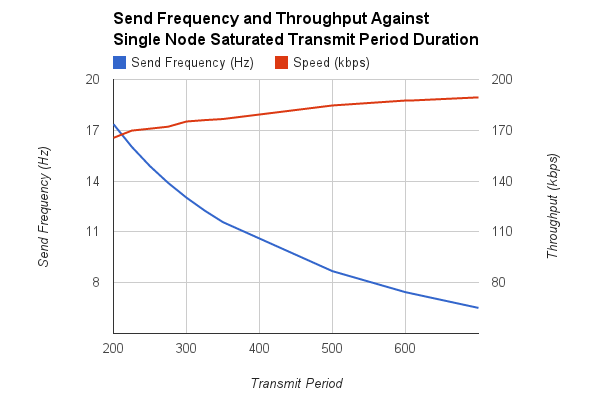
\includegraphics[width=120mm]{sendfreqvsthroughput.png}
	\caption{The Effects of Transmit Period on Latency and Throughput.}
	\label{fig:SendFreqVsThroughput}
\end{figure}

In Figure~\ref{fig:SendFreqVsThroughput} it can be seen that the throughput increases as the transmit period increases. This is to be expected as the guard periods are a fixed overhead, as the transmit period increases the ratio of guard period to transmit period moves in favour of the transmit period. Figure~\ref{fig:SendFreqVsThroughput} illustrates a 66.7 per cent decrease in send frequency against an 14.7 per cent increase in throughput. As in most applications of this technology the latency is a more important factor than throughput it is clear that a shorter transmit period is preferable. Figure~\ref{fig:ThroughputVsSendFreq} highlights the direct relationship between send frequency and throughput. The configuration used for these experiment was designed for the 4 producing nodes with 4 unreserved slots.

\begin{figure}
	\centering
	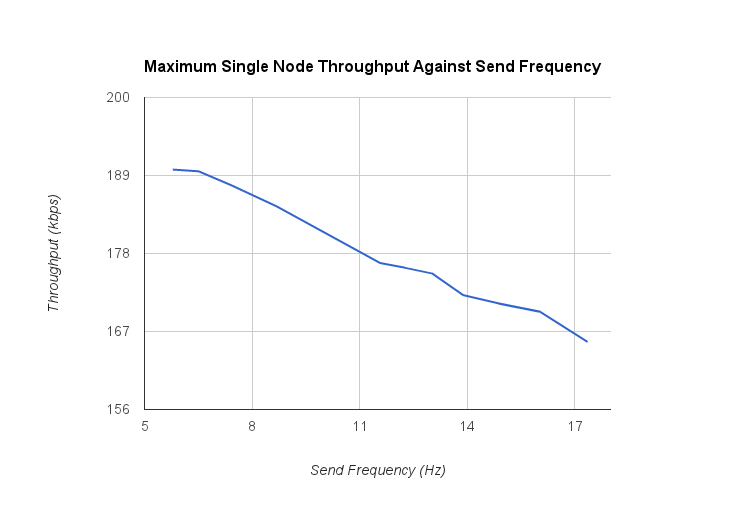
\includegraphics[width=120mm]{throughputvssendfreq.png}
	\caption{The Effect of Send Frequency on Throughput.}
	\label{fig:ThroughputVsSendFreq}
\end{figure}

A suitable transmit period of 300 for the following experiments has been selected. With this transmit period and a four node system with no unreserved slots a worst case latency for data being sent back is 42 ms. In contrast, if a transmit period of 900 ms had been chosen, in the same system there would be a latency of 107 ms. Whilst these are still fairly low, easily within the latency required for a good quality VoIP call for example, when unreserved slots are introduced in testing, this will increase dramatically. For instance, a 4 node system with 4 unreserved slots and a transmit period of 900 incurs a latency of 192 ms, around 5Hz. As opposed to a 300 transmit period which only incurs a latency of 76 ms with 4 unreserved slots.

\begin{figure}
	\centering
	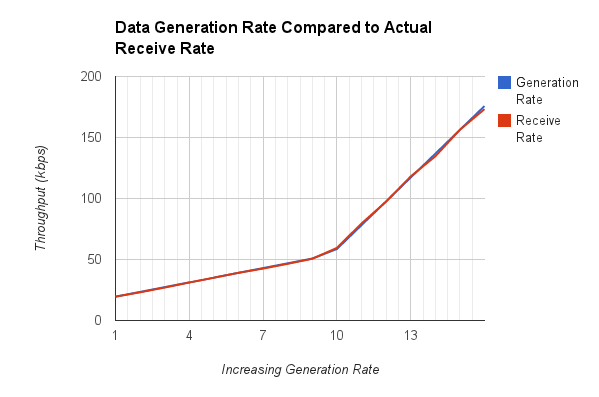
\includegraphics[width=120mm]{generationvsactual.png}
	\caption{Data Generation and Receive Rates.}
	\label{fig:GenerationVsActual}
\end{figure}

The performance of the unreserved slots can also be highlighted in a single node configuration. Figure~\ref{fig:GenerationVsActual} illustrates the change in throughput as the data generation rate increases for one node. It is clear that there are 2 major sections to the graph and 1 transitional state. The first section concerns the throughput up to 50 kbps. In this section the node is not using the full bandwidth available from its reserved slot. Above 60 kbps the node is making use of the allocated slots from the unreserved section. A higher throughput is seen as the node can continue to transmit through the guard periods in the unreserved section, an efficiency which is clearly exploited here. The transitional state occurs when the node is allocated only 1 slot from the unreserved section, in this state the node has a higher throughput per TDMA frame but does not benefit from the ability to transmit through guard periods. It is clear from this graph that the protocol is acting as expected, allocating more bandwidth to the node as required.

\subsection{ARQ Optimisations}

The most significant part of the ARQ are the optimisations which attempt to improve throughput while reducing the number of slots required. The optimisations are twofold; the ARQ attempts to reserve more slots if more packets are being queued than sucessfully sent and limits the maximum TDMA frame size if less than half the packets sent are accepted. The maximum frame size in this case is the number of consecutive data packets which can be transmitted by the node. When the node has reached the maximum TDMA frame size it begins resending the packets, similarly to the paper by Yao discussed in the related work \cite{PR6}. In particularly lossy channels this attempts to ensure optimum use of the allocated bandwidth by minimising the number of discarded packets at the base station. The effect of the optimisations on the throughput is illustrated by Figure~\ref{fig:ThroughputVsPacketLossOpt}. It is clear that the optimisations improve throughput through the whole range of packet loss, but the most significant efficiency is for packet loss less than 20 per cent. In the region of less than 10 per cent there is a greater than 50 per cent increase in throughput. 

\begin{figure}
	\centering
	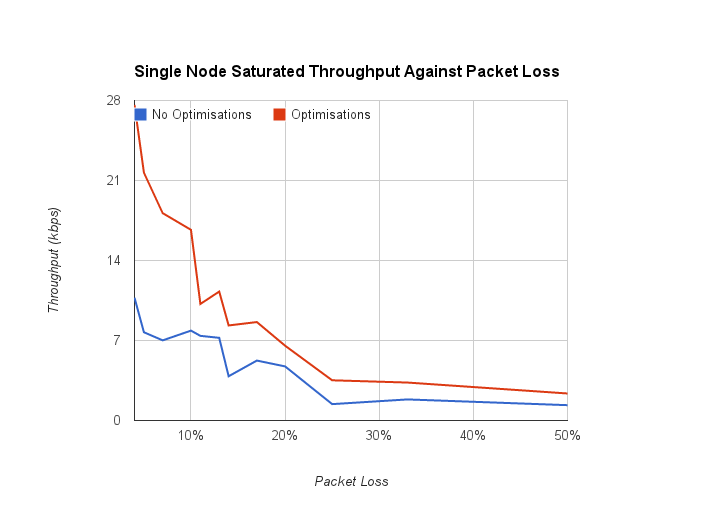
\includegraphics[width=120mm]{throughputvspacketlossopt.png}
	\caption{The Effect of Optimisations on Throughput.}
	\label{fig:ThroughputVsPacketLossOpt}
\end{figure}

\subsection{Unreserved Slots}

Figures~\ref{fig:ThroughputVsTransmitPeriod2} and~\ref{fig:ThroughputVsTransmitPeriod4} show the baseline throughput for 2 and 4 node systems with no optimisations or unreserved slots for nodes to request. These illustrate the maximum possible throughput for these systems, in ideal conditions (no packet loss) and saturated buffers (maximum possible data generation rate). While these do represent an ideal situation the next step is to consider the effect of packet loss on these systems. 

\begin{figure}
	\centering
	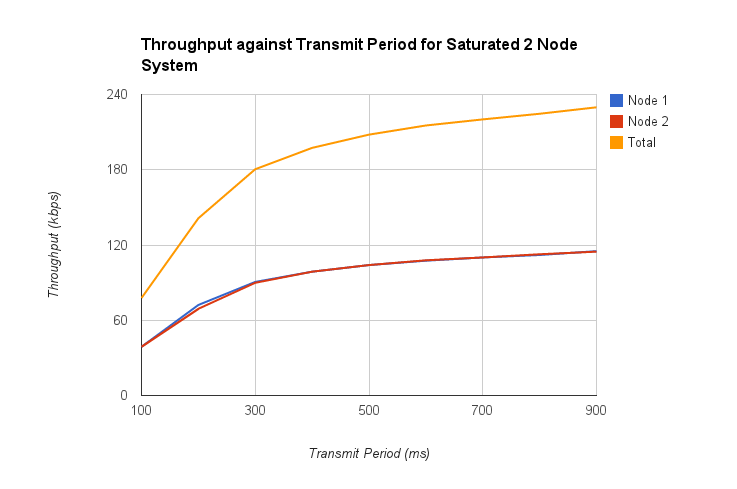
\includegraphics[width=120mm]{throughputvstransmitperiod2.png}
	\caption{Throughput in 2 Node System with no Optimisations or Unreserved Slots.}
	\label{fig:ThroughputVsTransmitPeriod2}
\end{figure}

\begin{figure}
	\centering
	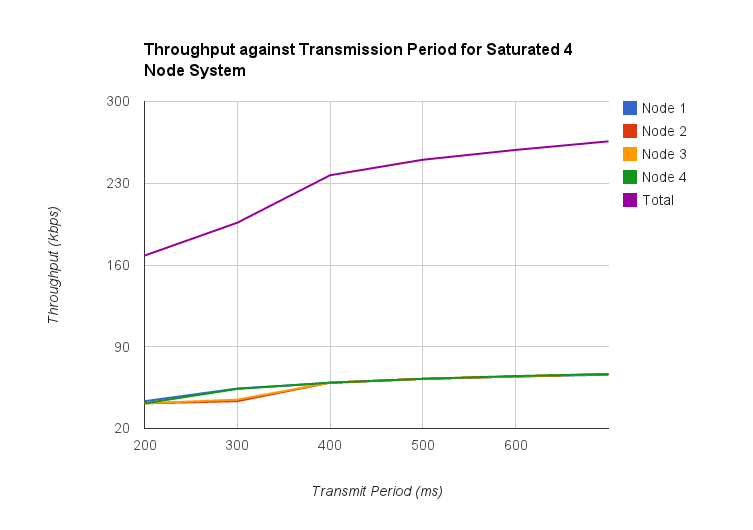
\includegraphics[width=120mm]{throughputvstransmitperiod4.png}
	\caption{Throughput in 4 Node System with no Optimisations or Unreserved Slots.}
	\label{fig:ThroughputVsTransmitPeriod4}
\end{figure}

Figures~\ref{fig:ThroughputVsLoss} and~\ref{fig:ThroughputVsLossOpt} illustrate the throughput change with varying packet loss, this test utilised saturated buffers to maximise throughput. It is clear that the optimisations provide higher throughput for the transmission time provided. The largest improvements are in the packet loss region of 20 to 40 per cent. For packet loss up to 20 per cent the optimisations provide neither significant improvement or detriment to the total throughput. If Figure~\ref{fig:ThroughputVsPacketLossOpt} is now considered, which illustrates the improvement provided by the optimisations on the total throughput for both systems, it can be seen that there is increased throughput with optimisations.

\begin{figure}
	\centering
	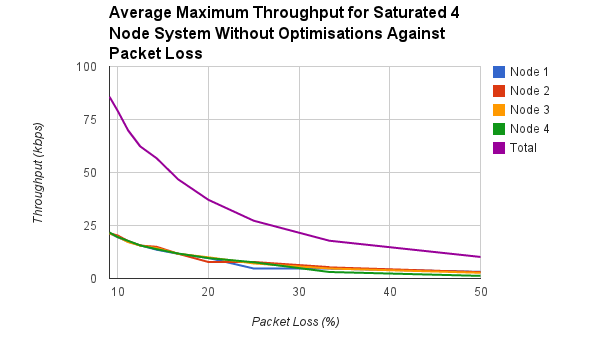
\includegraphics[width=120mm]{throughputvsloss.png}
	\caption{Throughput with Varying Packet Loss for 4 node System.}
	\label{fig:ThroughputVsLoss}
\end{figure}

\begin{figure}
	\centering
	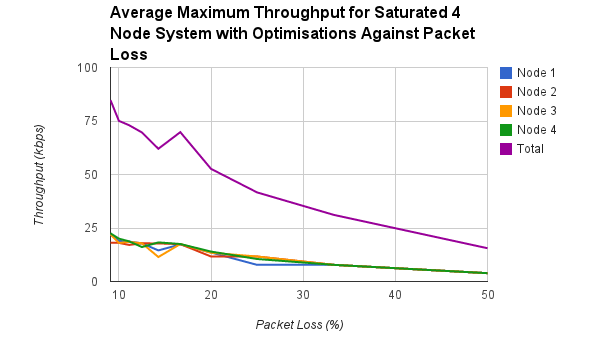
\includegraphics[width=120mm]{throughputvslossopt.png}
	\caption{Throughput with Varying Packet Loss for 4 node System with Optimisations.}
	\label{fig:ThroughputVsLossOpt}
\end{figure}

Figure~\ref{fig:ThroughputVsSlotCount4} actually shows a decrease in overall throughput for a four node system with packet loss. In this case a packet loss of 33 per cent was used with a fixed data generation rate of 50 kbps (around the maximum data rate possible for a 4 node system in ideal conditions). Using this data generation rate causes the nodes buffers to saturate, and therefore it can be seen that there is a higher throughput most similar to a configuration in which nodes are unable to transmit as fast as their generated data. The main trend shown in the graph of decreasing data rate against increasing number of slots is due to the extra overhead of each additional slot. As each slot requires a guard period, regardless of whether this slot and the preceding one are allocated and therefore transmission can occur through the guard period there will always be at most n additional guard periods (for a system with n nodes) which are being observed in the unreserved slot region as at most each node may be allocated one extra slot. The other contributing factor to decreased data rate is that as the slot count increases, the frequency at which the reserved slots are utilised is also decreased. In a 4 node system with a transmit period of 300 and 8 unreserved slots it can be seen that the frequency of TDMA frames to be 9 Hz, much less than in the same system with no unreserved slots of 23 Hz.

\begin{figure}
	\centering
	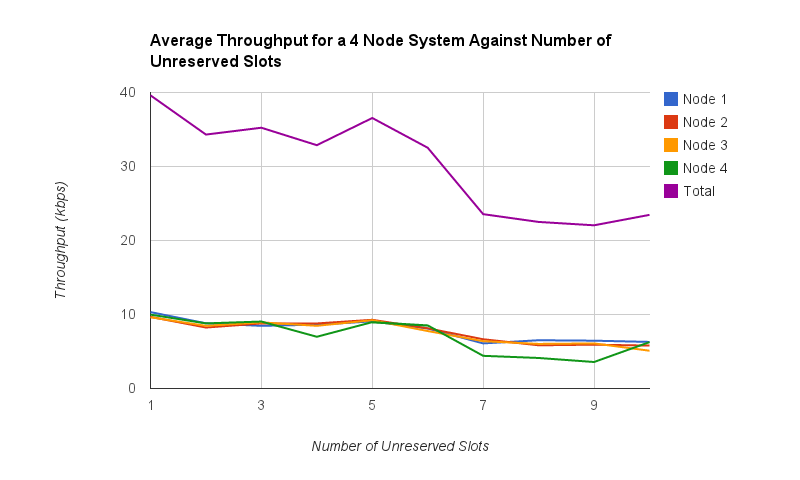
\includegraphics[width=120mm]{throughputvsslotcount4.png}
	\caption{Average Throughput for Varying Numbers of Unreserved Slots.}
	\label{fig:ThroughputVsSlotCount4}
\end{figure}

It follows from this to consider the performance of a system with nodes sending different, lower, rates of data over a lossy channel with nodes generating varying amounts of data. In this case a 4 node system with nodes generating different data at different rates will be used. Again differing levels of packet loss will be introduced to investigate the effects of packet loss on throughput. Figures~\ref{fig:ThroughputVsLossGen} and~\ref{fig:ThroughputVsLossGenSlots} make it clear that in a 4 node system, as expected from previous results, there is a higher total throughput for the system without unreserved slots as opposed to reserved slots. The decrease in bandwidth is probably from the overheads incurred of unreserved slots. 

\begin{figure}
	\centering
	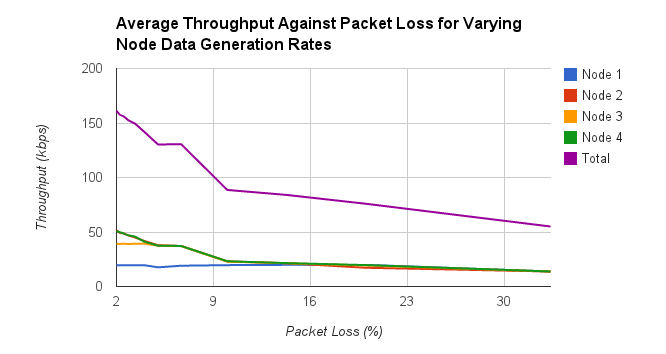
\includegraphics[width=120mm]{throughputvslossvaryinggeneration.png}
	\caption{Throughput for Varying Packet Loss with a Range of Data Generation Rates.}
	\label{fig:ThroughputVsLossGen}
\end{figure}

\begin{figure}
	\centering
	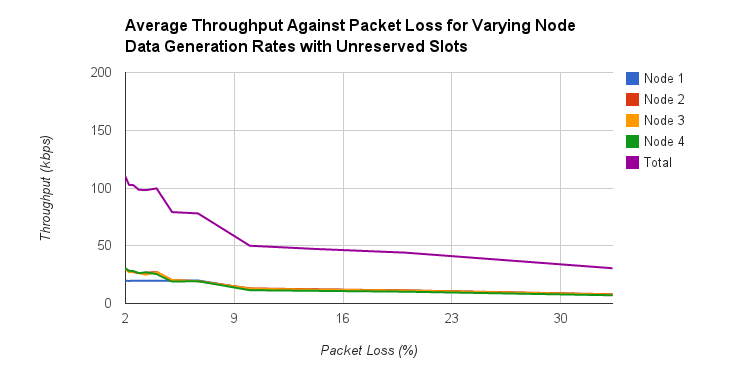
\includegraphics[width=120mm]{throughputvslossvaryinggenerationslots.png}
	\caption{Throughput for Varying Packet Loss with a Range of Data Generation Rates and Unreserved Slots.}
	\label{fig:ThroughputVsLossGenSlots}
\end{figure}

\chapter{Conclusion \& Further Work}

\section{Conclusion}

The novel solution proposed to improve throughput by including unreserved slots in the TDMA frame has been shown to have a detrimental effect on the total throughput of multiple node systems. The optimisations to the ARQ sub-protocol do show strong improvements on the baseline results under lossy conditions. As the main goal of the project is to research and develop a protocol utilising dynamically allocatable TDMA slots to provide delivery guarantees over a lossy radio connection for the context of real time sensor networks (specifically motion capture, in which latency and throughput are the most important factors) these constraints must be accounted for when considering the conclusions of the project. 

The ARQ sub-protocol optimisations show good throughput gain in lossy conditions, utilising the preassigned bandwidth. The optimisations require no additional overheads related to the bandwidth available to the node and purely aim to maximise the number of sequential packets received successfully by the base station. The optimisations highlight the downside of using a Go Back-N inspired ARQ sub-protocol to provide delivery guarantees, however it should be noted that the motivation for this choice was indeed the bandwidth requirements of the base station sending acknowledgements to nodes.

The novel extension of a static TDMA algorithm to include unreserved slots dynamically allocated to nodes in need of extra bandwidth in this instance did not show any improvement on the static TDMA implementation it was compared to. Additionally the extra slots actually have a relatively high overhead and therefore cost to the TDMA throughput and latency. As these are potentially the most important factors in the context described, the ARQ algorithm may need to be reengineered to send the most recently produced data first, whilst still being able to send back older data to ensure at the end of a capture the complete data set is transferred to the base station. 

If the original context of the project is considered, a motion capture on a swimmer, the proposed protocol will perform well. While the nodes are under the water there will be no communication due to the frequency of communication (2.4 GHz in this case) and so there is no protocol which can recover this data until the node surfaces. If some nodes are out of the water for most of their operation, data will be retrieved normally. If a node appears out of the water for a short period it may benefit from the unreserved slots, provided it is out of the water for long enough. For instance, if, in a typical 16 node system with 4 unreserved slots, a node is out of the water for more than 360 ms it will transmit data to the base station. If the node is out of the water for more than 540 ms it will benefit from extra slots though these may already be contested. The main benefit will be when the swimmer leaves the water. In this case there will be a low packet loss and the protocol will take advantage of this, transmitting data with a higher throughput than a simple TDMA based algorithm.

The main conclusion which can be drawn from the results presented, is that the best way to provide an efficient radio connection over lossy channel, in this context, is to provide sufficient bandwidth to all nodes for their radio nodes from the initialisation of the protocol. The novel solution investigated in this project appears to have a detrimental effect. As nodes transition between being in and out of range it is not feasible to make changes to the underlying TDMA configurations at run time without consensus from all participating nodes. The required consensus may take many TDMA frames to achieve (especially if multiple nodes are not within radio range or transmitting over particularly lossy channels) and as a result the time required to make these changes is expected to have a higher relative detrimental effect on network performance than pre-assigning ample bandwidth. The overheads of providing extra slots have been shown to have a detrimental effect on the latency and total throughput of the network which, in the context of real time sensing, could make the network unable to fulfill expectations. When choosing suitable suitable parameters for the TDMA configuration it would be best to consider the expected and observed packet loss along with expected data generation rates and maximum latency. It has been shown that higher throughput can be achieved if very low latency is not an absolute requirement.

\newpage
\section{Further Work}

It may not be feasible to propose and develop a new protocol for each instance of data recovery in hostile environment and it is clear that the proposed protocol is not a fix-all solution. Hostile environments vary greatly in their effects on overall packet loss, radio reception and data generation rates. If the application has a minimum bandwidth requirement greater than the maximum available bandwidth, no protocol design will be able to meet expectations. 

The next step into research of the protocol presented would be to consider the concept of priorities when allocating slots. Nodes request slots for multiple reasons and currently all slot requests are considered equally. By introducing priorities bandwidth requirements may be balanced more fairly. This concept was experimented with, by spreading the node generation rates, nodes request slots when required. Implementation of an allocation module capable of extensible prioritising to be performed on the base station node would require extensive development time. It is not known whether it is possible to implement this allocation algorithm without detrimental effects on the performance of the TDMA on the nodes. 

A possible solution to understanding a specific hostile environment and optimising a protocol to maximise throughput could be developed through profiling. Profiling of an environment would involve performing a series of trial runs of an experiment. Through analysing packet drop, ARQ optimisations (such as maximum frame size) and overall throughput, suitable TDMA configurations can be created. This could then be extended to multiple configurations per experiment. Each configuration can be given a validity period, bound by two TDMA frame numbers. Provided nodes have knowledge of which TDMA frame is current, the correct configuration can be selected. The reference packet used for synchronisation can be extended to include the current TDMA frame number, ensuring synchronisation between all nodes when they are active (i.e. within radio range of the base station). It is expected that configurations will instruct nodes of their slot start and duration, as well as the possibility to control variables related to the ARQ optimisations. Examples of controllable ARQ optimisations include when to impose a maximum frame size and how to decide this value. 

Throughout the project the assumption that it is most important for all generated data to be guaranteed delivery has motivated the ARQ selection and its implementation. An alternative scenario should be considered in which receiving enough data to update a real time model is the most important objective. An example of this requirement is a motion capture with real time output, such as an avatar mimicking the actions of a person. If these data requirements are acceptable, the required bandwidth of the system is reduced. A reduced bandwidth requirement means protocols stand a better chance of successfully transmitting current data. 

Finally a further study of the effects of TDMA based protocols on battery health and discharge time may raise key points of discussion as to whether TDMA based algorithms are suitable for sensor networks with high throughput or packet loss. It is known that periods of high current draw have detrimental effects on battery health, in the case of TDMA based algorithms each transmit period is optimised to ensure the node transmits as many packets as possible (i.e. maximise throughput). As a result of this, the protocol presented may actually cause harm to the internal chemical reactions of the batteries. 


% use the following and \cite{} as above if you use BibTeX
% otherwise generate bibtem entries
\bibliographystyle{plain}
\bibliography{mybibfile}

\appendix
\chapter{Sample Base Station Log}

build complete\newline
enable node [nid=1,txp=300,loss=0,optimisations=0,dataRate=0,slots=7]\newline
0[211]: aloha tx mode\newline
0[211]: packet sent\newline
0[211]: aloha rx mode\newline
enable master [txp=300,reservedSlots=2,unreservedSlots=5,slotCount=7,lease=5]\newline
8[246]: last recv count = 22\newline
125[246]: lease: [nid=1,slotid=2,len=5,lease=1,ack=234]\newline
142[246]: send ack n:1 0/194\newline
158[246]: packet sent\newline
521[246]: packet received\newline
543[246]: packet received\newline
562[246]: packet received\newline
582[246]: packet received\newline
601[246]: packet received\newline
621[246]: packet received\newline
641[246]: packet received\newline
659[246]: packet received\newline
680[246]: packet received\newline
699[246]: packet received\newline
719[246]: packet received\newline
739[246]: packet received\newline
759[246]: packet received\newline
921[246]: packet received\newline
941[246]: packet received\newline
961[246]: packet received\newline
981[246]: packet received\newline
999[246]: packet received\newline
1020[246]: packet received\newline
1039[246]: packet received\newline
1060[246]: packet received\newline
1079[246]: packet received\newline
1098[246]: packet received\newline
9[247]: last recv count = 24\newline
125[247]: lease: [nid=1,slotid=2,len=5,lease=1,ack=235]\newline
142[247]: send ack n:1 3/199\newline
158[247]: packet sent\newline
520[247]: packet received\newline
541[247]: packet received\newline
559[247]: packet received\newline
580[247]: packet received\newline
599[247]: packet received\newline
619[247]: packet received\newline
638[247]: packet received\newline
658[247]: packet received\newline
677[247]: packet received\newline
697[247]: packet received\newline
716[247]: packet received\newline
735[247]: packet received\newline
756[247]: packet received\newline
775[247]: packet received\newline
920[247]: packet received\newline
940[247]: packet received\newline
960[247]: packet received\newline
980[247]: packet received\newline
998[247]: packet received\newline
1019[247]: packet received\newline
1039[247]: packet received\newline
1057[247]: packet received\newline
1078[247]: packet received\newline
1098[247]: packet received\newline
1118[247]: packet received\newline
1138[247]: packet received\newline
1158[247]: packet received\newline
1176[247]: packet received\newline
1196[247]: packet received\newline
1216[247]: packet received\newline
1234[247]: packet received\newline
1254[247]: packet received\newline
8[248]: last recv count = 33\newline
125[248]: lease: [nid=1,slotid=2,len=5,lease=1,ack=236]\newline
142[248]: send ack n:1 3/207\newline
159[248]: packet sent\newline
521[248]: packet received\newline
542[248]: packet received\newline
561[248]: packet received\newline
581[248]: packet received\newline
600[248]: packet received\newline
620[248]: packet received\newline
641[248]: packet received\newline
660[248]: packet received\newline
678[248]: packet received\newline
698[248]: packet received\newline
718[248]: packet received\newline
737[248]: packet received\newline
757[248]: packet received\newline
776[248]: packet received\newline
921[248]: packet received\newline
941[248]: packet received\newline
960[248]: packet received\newline
980[248]: packet received\newline
1001[248]: packet received\newline
1020[248]: packet received\newline
8[249]: last recv count = 21\newline
125[249]: lease: [nid=1,slotid=2,len=5,lease=1,ack=237]\newline
142[249]: send ack n:1 3/212\newline
158[249]: packet sent\newline
521[249]: packet received\newline
541[249]: packet received\newline
561[249]: packet received\newline
581[249]: packet received\newline
599[249]: packet received\newline
620[249]: packet received\newline
639[249]: packet received\newline
659[249]: packet received\newline
678[249]: packet received\newline
699[249]: packet received\newline
719[249]: packet received\newline
8[250]: last recv count = 12\newline
125[250]: lease: [nid=1,slotid=2,len=5,lease=1,ack=238]\newline
143[250]: send ack n:1 2/215\newline
159[250]: packet sent\newline
521[250]: packet received\newline
541[250]: packet received\newline
561[250]: packet received\newline
581[250]: packet received\newline
600[250]: packet received\newline
620[250]: packet received\newline
640[250]: packet received\newline
660[250]: packet received\newline
679[250]: packet received\newline
699[250]: packet received\newline
718[250]: packet received\newline
738[250]: packet received\newline
756[250]: packet received\newline
921[250]: packet received\newline
940[250]: packet received\newline
961[250]: packet received\newline
980[250]: packet received\newline
1000[250]: packet received\newline
1020[250]: packet received\newline
1039[250]: packet received\newline
1059[250]: packet received\newline
8[251]: last recv count = 22\newline
125[251]: lease: [nid=1,slotid=2,len=5,lease=1,ack=239]\newline
143[251]: send ack n:1 3/220\newline
158[251]: packet sent\newline
521[251]: packet received\newline
541[251]: packet received\newline
561[251]: packet received\newline
580[251]: packet received\newline
602[251]: packet received\newline
621[251]: packet received\newline
640[251]: packet received\newline
661[251]: packet received\newline
680[251]: packet received\newline
699[251]: packet received\newline
720[251]: packet received\newline
740[251]: packet received\newline
758[251]: packet received\newline
8[252]: last recv count = 14\newline

\chapter{Sample Node Log Without Slots}

0[707]: packet received\newline
0[707]: packet received\newline
2[707]: tdma started\newline
9[707]: packet loss: 0\newline
16[707]: improvements: disabled\newline
25[707]: data rate: auto\newline
138[707]: timing packet found\newline
3[708]: last send count = 4\newline
3[709]: last send count = 0\newline
3[710]: last send count = 0\newline
3[711]: last send count = 0\newline
0[711]: tdma out of sync\newline
2[711]: tdma started\newline
109[711]: timing packet found\newline
3[712]: last send count = 0\newline
116[712]: sync complete\newline
\newline
130[712]: packet received\newline
139[712]: packet received\newline
149[712]: sync packet found\newline
501[712]: sending packets\newline
520[712]: packet sent\newline
540[712]: packet sent\newline
559[712]: packet sent\newline
579[712]: packet sent\newline
599[712]: packet sent\newline
618[712]: packet sent\newline
638[712]: packet sent\newline
657[712]: packet sent\newline
677[712]: packet sent\newline
696[712]: packet sent\newline
716[712]: packet sent\newline
736[712]: packet sent\newline
756[712]: packet sent\newline
765[712]: protection period start\newline
1[713]: end transmission period\newline
13[713]: last send count = 14\newline
119[713]: packet received\newline
128[713]: packet received\newline
137[713]: sync packet found\newline
154[713]: packet received\newline
162[713]: packet received\newline
185[713]: sent 14 packets 986 remaining [ack 1/3] [maxFrameSize=0]\newline
501[713]: sending packets\newline
520[713]: packet sent\newline
539[713]: packet sent\newline
560[713]: packet sent\newline
579[713]: packet sent\newline
599[713]: packet sent\newline
619[713]: packet sent\newline
638[713]: packet sent\newline
658[713]: packet sent\newline
677[713]: packet sent\newline
697[713]: packet sent\newline
716[713]: packet sent\newline
735[713]: packet sent\newline
755[713]: packet sent\newline
765[713]: protection period start\newline
1[714]: end transmission period\newline
13[714]: last send count = 15\newline
119[714]: packet received\newline
128[714]: packet received\newline
137[714]: sync packet found\newline
154[714]: packet received\newline
162[714]: packet received\newline
185[714]: sent 14 packets 988 remaining [ack 3/6] [maxFrameSize=0]\newline
501[714]: sending packets\newline
521[714]: packet sent\newline
540[714]: packet sent\newline
560[714]: packet sent\newline
579[714]: packet sent\newline
599[714]: packet sent\newline
618[714]: packet sent\newline
638[714]: packet sent\newline
657[714]: packet sent\newline
677[714]: packet sent\newline
696[714]: packet sent\newline
716[714]: packet sent\newline
735[714]: packet sent\newline
755[714]: packet sent\newline
765[714]: protection period start\newline
1[715]: end transmission period\newline
13[715]: last send count = 15\newline
119[715]: packet received\newline
127[715]: packet received\newline
137[715]: sync packet found\newline
153[715]: packet received\newline
162[715]: packet received\newline
186[715]: sent 14 packets 986 remaining [ack 1/10] [maxFrameSize=0]\newline
501[715]: sending packets\newline
520[715]: packet sent\newline
540[715]: packet sent\newline
559[715]: packet sent\newline
579[715]: packet sent\newline
598[715]: packet sent\newline
618[715]: packet sent\newline
637[715]: packet sent\newline
657[715]: packet sent\newline
677[715]: packet sent\newline
696[715]: packet sent\newline
715[715]: packet sent\newline
735[715]: packet sent\newline
755[715]: packet sent\newline
764[715]: protection period start\newline
1[716]: end transmission period\newline

\chapter{Sample Node Log With Unreserved Slots}

0[0]: packet received\newline
0[0]: packet received\newline
2[0]: tdma started\newline
6[0]: packet loss: 0\newline
11[0]: improvements: disabled\newline
18[0]: data rate: auto\newline
128[0]: timing packet found\newline
3[1]: last send count = 1\newline
116[1]: sync complete\newline
\newline
128[1]: packet received\newline
134[1]: packet received\newline
142[1]: sync packet found\newline
501[1]: sending packets\newline
520[1]: packet sent\newline
540[1]: packet sent\newline
560[1]: packet sent\newline
579[1]: packet sent\newline
599[1]: packet sent\newline
618[1]: packet sent\newline
638[1]: packet sent\newline
658[1]: packet sent\newline
677[1]: packet sent\newline
697[1]: packet sent\newline
716[1]: packet sent\newline
736[1]: packet sent\newline
755[1]: packet sent\newline
762[1]: protection period start\newline
802[1]: end transmission period\newline
4[2]: last send count = 14\newline
120[2]: packet received\newline
126[2]: packet received\newline
133[2]: sync packet found\newline
166[2]: packet received\newline
173[2]: packet received\newline
193[2]: sent 14 packets 986 remaining [ack 1/3] [maxFrameSize=0]\newline
204[2]: slot lease [start slot=2,length=1,lease remaining=5]\newline
501[2]: sending packets\newline
520[2]: packet sent\newline
540[2]: packet sent\newline
559[2]: packet sent\newline
579[2]: packet sent\newline
598[2]: packet sent\newline
618[2]: packet sent\newline
638[2]: packet sent\newline
657[2]: packet sent\newline
677[2]: packet sent\newline
696[2]: packet sent\newline
716[2]: packet sent\newline
736[2]: packet sent\newline
756[2]: packet sent\newline
763[2]: protection period start\newline
802[2]: end transmission period\newline
901[2]: sending packets\newline
920[2]: packet sent\newline
940[2]: packet sent\newline
959[2]: packet sent\newline
979[2]: packet sent\newline
999[2]: packet sent\newline
1018[2]: packet sent\newline
1038[2]: packet sent\newline
1057[2]: packet sent\newline
1076[2]: packet sent\newline
1096[2]: packet sent\newline
1115[2]: packet sent\newline
1135[2]: packet sent\newline
1155[2]: packet sent\newline
1162[2]: protection period start\newline
1201[2]: end transmission period\newline
4[3]: last send count = 28\newline
120[3]: packet received\newline
126[3]: packet received\newline
133[3]: sync packet found\newline
166[3]: packet received\newline
173[3]: packet received\newline
194[3]: sent 23 packets 979 remaining [ack 0/9] [maxFrameSize=0]\newline
204[3]: slot lease [start slot=2,length=2,lease remaining=4]\newline
501[3]: sending packets\newline
520[3]: packet sent\newline
540[3]: packet sent\newline
560[3]: packet sent\newline
579[3]: packet sent\newline
599[3]: packet sent\newline
618[3]: packet sent\newline
638[3]: packet sent\newline
657[3]: packet sent\newline
677[3]: packet sent\newline
697[3]: packet sent\newline
716[3]: packet sent\newline
736[3]: packet sent\newline
756[3]: packet sent\newline
762[3]: protection period start\newline
802[3]: end transmission period\newline
901[3]: sending packets\newline
920[3]: packet sent\newline
940[3]: packet sent\newline
960[3]: packet sent\newline
979[3]: packet sent\newline
999[3]: packet sent\newline
1018[3]: packet sent\newline
1038[3]: packet sent\newline
1057[3]: packet sent\newline
1077[3]: packet sent\newline
1096[3]: packet sent\newline
1115[3]: packet sent\newline
1135[3]: packet sent\newline
1154[3]: packet sent\newline
1174[3]: packet sent\newline
1194[3]: packet sent\newline
1213[3]: packet sent\newline
1232[3]: packet sent\newline
1252[3]: packet sent\newline
1271[3]: packet sent\newline
1291[3]: packet sent\newline
1310[3]: packet sent\newline
1330[3]: packet sent\newline
1349[3]: packet sent\newline
1369[3]: packet sent\newline
1388[3]: packet sent\newline
1408[3]: packet sent\newline
1428[3]: packet sent\newline
1447[3]: packet sent\newline
1467[3]: packet sent\newline
1486[3]: packet sent\newline
1505[3]: packet sent\newline
1525[3]: packet sent\newline
1545[3]: packet sent\newline
1552[3]: protection period start\newline
1602[3]: end transmission period\newline
4[4]: last send count = 48\newline
120[4]: packet received\newline
126[4]: packet received\newline
134[4]: sync packet found\newline
168[4]: packet received\newline
174[4]: packet received\newline
202[4]: sent 48 packets 955 remaining [ack 0/21] [maxFrameSize=0]\newline
212[4]: slot lease [start slot=2,length=3,lease remaining=3]\newline
501[4]: sending packets\newline
520[4]: packet sent\newline
540[4]: packet sent\newline
559[4]: packet sent\newline
579[4]: packet sent\newline
599[4]: packet sent\newline
618[4]: packet sent\newline
638[4]: packet sent\newline
657[4]: packet sent\newline
677[4]: packet sent\newline
696[4]: packet sent\newline
716[4]: packet sent\newline
736[4]: packet sent\newline
756[4]: packet sent\newline
762[4]: protection period start\newline
802[4]: end transmission period\newline
901[4]: sending packets\newline
920[4]: packet sent\newline
939[4]: packet sent\newline
959[4]: packet sent\newline
978[4]: packet sent\newline
998[4]: packet sent\newline
1018[4]: packet sent\newline
1037[4]: packet sent\newline
1057[4]: packet sent\newline
1076[4]: packet sent\newline
1095[4]: packet sent\newline
1115[4]: packet sent\newline
1134[4]: packet sent\newline
1154[4]: packet sent\newline
1173[4]: packet sent\newline
1193[4]: packet sent\newline
1212[4]: packet sent\newline
1231[4]: packet sent\newline
1251[4]: packet sent\newline
1271[4]: packet sent\newline
1290[4]: packet sent\newline
1310[4]: packet sent\newline
1329[4]: packet sent\newline
1349[4]: packet sent\newline
1368[4]: packet sent\newline
1388[4]: packet sent\newline
1407[4]: packet sent\newline
1427[4]: packet sent\newline
1446[4]: packet sent\newline
1466[4]: packet sent\newline
1485[4]: packet sent\newline
1505[4]: packet sent\newline
1524[4]: packet sent\newline
1544[4]: packet sent\newline
1563[4]: packet sent\newline
1583[4]: packet sent\newline
1603[4]: packet sent\newline
1622[4]: packet sent\newline
1642[4]: packet sent\newline
1661[4]: packet sent\newline
1681[4]: packet sent\newline
1700[4]: packet sent\newline
1720[4]: packet sent\newline
1740[4]: packet sent\newline
1759[4]: packet sent\newline
1779[4]: packet sent\newline
1798[4]: packet sent\newline
1818[4]: packet sent\newline
1838[4]: packet sent\newline
1857[4]: packet sent\newline
1877[4]: packet sent\newline
1896[4]: packet sent\newline
1916[4]: packet sent\newline
1935[4]: packet sent\newline
1956[4]: packet sent\newline
1963[4]: protection period start\newline
2002[4]: end transmission period\newline
5[5]: last send count = 69\newline
120[5]: packet received\newline
126[5]: packet received\newline
133[5]: sync packet found\newline
168[5]: packet received\newline
174[5]: packet received\newline
205[5]: sent 69 packets 934 remaining [ack 1/38] [maxFrameSize=0]\newline
216[5]: slot lease [start slot=2,length=4,lease remaining=2]\newline
501[5]: sending packets\newline
520[5]: packet sent\newline
540[5]: packet sent\newline
560[5]: packet sent\newline
579[5]: packet sent\newline
599[5]: packet sent\newline
618[5]: packet sent\newline
638[5]: packet sent\newline
658[5]: packet sent\newline
677[5]: packet sent\newline
697[5]: packet sent\newline
716[5]: packet sent\newline
736[5]: packet sent\newline
755[5]: packet sent\newline
762[5]: protection period start\newline
802[5]: end transmission period\newline
901[5]: sending packets\newline
920[5]: packet sent\newline
939[5]: packet sent\newline
959[5]: packet sent\newline
979[5]: packet sent\newline
998[5]: packet sent\newline
1017[5]: packet sent\newline
1037[5]: packet sent\newline
1056[5]: packet sent\newline
1076[5]: packet sent\newline
1095[5]: packet sent\newline
1115[5]: packet sent\newline
1134[5]: packet sent\newline
1154[5]: packet sent\newline
1173[5]: packet sent\newline
1193[5]: packet sent\newline
1212[5]: packet sent\newline
1232[5]: packet sent\newline
1251[5]: packet sent\newline
1271[5]: packet sent\newline
1290[5]: packet sent\newline
1310[5]: packet sent\newline
1329[5]: packet sent\newline
1349[5]: packet sent\newline
1368[5]: packet sent\newline
1388[5]: packet sent\newline
1407[5]: packet sent\newline
1427[5]: packet sent\newline
1446[5]: packet sent\newline
1466[5]: packet sent\newline
1485[5]: packet sent\newline
1505[5]: packet sent\newline
1524[5]: packet sent\newline
1544[5]: packet sent\newline
1564[5]: packet sent\newline
1583[5]: packet sent\newline
1602[5]: packet sent\newline
1622[5]: packet sent\newline
1642[5]: packet sent\newline
1661[5]: packet sent\newline
1681[5]: packet sent\newline
1701[5]: packet sent\newline
1720[5]: packet sent\newline
1740[5]: packet sent\newline
1759[5]: packet sent\newline
1779[5]: packet sent\newline
1799[5]: packet sent\newline
1818[5]: packet sent\newline
1838[5]: packet sent\newline
1857[5]: packet sent\newline
1877[5]: packet sent\newline
1896[5]: packet sent\newline
1916[5]: packet sent\newline
1936[5]: packet sent\newline
1955[5]: packet sent\newline
1975[5]: packet sent\newline
1994[5]: packet sent\newline
2014[5]: packet sent\newline
2034[5]: packet sent\newline
2053[5]: packet sent\newline
2073[5]: packet sent\newline
2092[5]: packet sent\newline
2112[5]: packet sent\newline
2131[5]: packet sent\newline
2151[5]: packet sent\newline
2170[5]: packet sent\newline
2190[5]: packet sent\newline
2210[5]: packet sent\newline
2229[5]: packet sent\newline
2249[5]: packet sent\newline
2269[5]: packet sent\newline
2288[5]: packet sent\newline
2308[5]: packet sent\newline
2327[5]: packet sent\newline
2347[5]: packet sent\newline
2355[5]: protection period start\newline
2402[5]: end transmission period\newline
4[6]: last send count = 89\newline
120[6]: packet received\newline
126[6]: packet received\newline
133[6]: sync packet found\newline
168[6]: packet received\newline
174[6]: packet received\newline
209[6]: sent 89 packets 913 remaining [ack 2/60] [maxFrameSize=0]\newline
220[6]: slot lease [start slot=2,length=5,lease remaining=1]\newline
501[6]: sending packets\newline
520[6]: packet sent\newline
540[6]: packet sent\newline
559[6]: packet sent\newline
579[6]: packet sent\newline
598[6]: packet sent\newline
618[6]: packet sent\newline
638[6]: packet sent\newline
657[6]: packet sent\newline
677[6]: packet sent\newline
696[6]: packet sent\newline
716[6]: packet sent\newline
736[6]: packet sent\newline
755[6]: packet sent\newline
763[6]: protection period start\newline
802[6]: end transmission period\newline
901[6]: sending packets\newline
920[6]: packet sent\newline
940[6]: packet sent\newline
959[6]: packet sent\newline
979[6]: packet sent\newline
998[6]: packet sent\newline
1018[6]: packet sent\newline
1037[6]: packet sent\newline
1057[6]: packet sent\newline
1076[6]: packet sent\newline
1095[6]: packet sent\newline
1115[6]: packet sent\newline
1134[6]: packet sent\newline
1154[6]: packet sent\newline
1173[6]: packet sent\newline
1193[6]: packet sent\newline
1212[6]: packet sent\newline
1232[6]: packet sent\newline
1251[6]: packet sent\newline
1271[6]: packet sent\newline
1290[6]: packet sent\newline
1310[6]: packet sent\newline
1329[6]: packet sent\newline
1349[6]: packet sent\newline
1368[6]: packet sent\newline
1388[6]: packet sent\newline
1407[6]: packet sent\newline
1427[6]: packet sent\newline
1446[6]: packet sent\newline
1466[6]: packet sent\newline
1485[6]: packet sent\newline
1505[6]: packet sent\newline
1524[6]: packet sent\newline
1544[6]: packet sent\newline
1563[6]: packet sent\newline
1583[6]: packet sent\newline
1603[6]: packet sent\newline
1622[6]: packet sent\newline
1642[6]: packet sent\newline
1661[6]: packet sent\newline
1681[6]: packet sent\newline
1700[6]: packet sent\newline
1720[6]: packet sent\newline
1739[6]: packet sent\newline
1759[6]: packet sent\newline
1779[6]: packet sent\newline
1798[6]: packet sent\newline
1818[6]: packet sent\newline
1837[6]: packet sent\newline
1857[6]: packet sent\newline
1877[6]: packet sent\newline
1896[6]: packet sent\newline
1916[6]: packet sent\newline
1935[6]: packet sent\newline
1955[6]: packet sent\newline
1974[6]: packet sent\newline
1994[6]: packet sent\newline
2013[6]: packet sent\newline
2033[6]: packet sent\newline
2053[6]: packet sent\newline
2072[6]: packet sent\newline
2092[6]: packet sent\newline
2112[6]: packet sent\newline
2131[6]: packet sent\newline
2151[6]: packet sent\newline
2170[6]: packet sent\newline
2190[6]: packet sent\newline
2209[6]: packet sent\newline
2229[6]: packet sent\newline
2248[6]: packet sent\newline
2268[6]: packet sent\newline
2288[6]: packet sent\newline
2307[6]: packet sent\newline
2327[6]: packet sent\newline
2347[6]: packet sent\newline
2366[6]: packet sent\newline
2386[6]: packet sent\newline
2405[6]: packet sent\newline
2425[6]: packet sent\newline
2444[6]: packet sent\newline
2464[6]: packet sent\newline
2483[6]: packet sent\newline
2503[6]: packet sent\newline
2522[6]: packet sent\newline
2542[6]: packet sent\newline
2562[6]: packet sent\newline
2581[6]: packet sent\newline
2601[6]: packet sent\newline
2620[6]: packet sent\newline
2640[6]: packet sent\newline
2659[6]: packet sent\newline
2679[6]: packet sent\newline
2699[6]: packet sent\newline
2718[6]: packet sent\newline
2738[6]: packet sent\newline
2751[6]: protection period start\newline
1[7]: end transmission period\newline

\end{document}
